%%%%%%%%%%%%%%%%%%%%%%%%%%%%%%%%%%%%%%%%%
% Professional Newsletter Template
% LaTeX Template
% Version 1.0 (09/03/14)
%
% Created by:
% Bob Kerstetter (https://www.tug.org/texshowcase/) and extensively modified by:
% Vel (vel@latextemplates.com)
% 
% This template has been downloaded from:
% http://www.LaTeXTemplates.com
%
% License:
% CC BY-NC-SA 3.0 (http://creativecommons.org/licenses/by-nc-sa/3.0/)
%
%%%%%%%%%%%%%%%%%%%%%%%%%%%%%%%%%%%%%%%%%

\documentclass[12pt]{article} % The default font size is 10pt; 11pt and 12pt are alternatives

%%%%%%%%%%%%%%%%%%%%%%%%%%%%%%%%%%%%%%%%%
% Professional Newsletter Template
% Structural Definitions File
% Version 1.0 (09/03/14)
%
% Created by:
% Vel (vel@latextemplates.com)
% 
% This file has been downloaded from:
% http://www.LaTeXTemplates.com
%
% License:
% CC BY-NC-SA 3.0 (http://creativecommons.org/licenses/by-nc-sa/3.0/)
%
%%%%%%%%%%%%%%%%%%%%%%%%%%%%%%%%%%%%%%%%%

%----------------------------------------------------------------------------------------
%	REQUIRED PACKAGES
%----------------------------------------------------------------------------------------

\usepackage{graphicx} % Required for including images
\usepackage{microtype} % Improved typography
\usepackage{multicol} % Used for the two-column layout of the document
\usepackage{booktabs} % Required for nice horizontal rules in tables
\usepackage{wrapfig} % Required for in-line images
\usepackage{float} % Required for forcing figures not to float with the [H] parameter
\usepackage[at]{easylist}                                        % Easy lists
\usepackage{microtype}                                                  % Niceness
\usepackage{anyfontsize}                                                  % Niceness

%------------------------------------------------
% Fonts

\usepackage{charter} % Use the Charter font as the main document font
\usepackage{courier} % Use the Courier font for \texttt (monospaced) only
\usepackage[T1]{fontenc} % Use T1 font encoding

%------------------------------------------------
% List Separation

\usepackage{enumitem} % Required to customize the list environments
\setlist{noitemsep,nolistsep} % Remove spacing before, after and within lists for a compact look

%------------------------------------------------
% Figure and Table Caption Styles

\usepackage{caption} % Required for changing caption styles
\captionsetup[table]{labelfont={bf,sf},labelsep=period,justification=justified} % Specify the table caption style
\captionsetup[figure]{labelfont={sf,bf},labelsep=period,justification=justified, font=small} % Specify the figure caption style
\setlength{\abovecaptionskip}{10pt} % Whitespace above captions

%------------------------------------------------
% Spacing Between Paragraphs

\makeatletter
\usepackage{parskip}
\setlength{\parskip}{6pt}
\newcommand{\@minipagerestore}{\setlength{\parskip}{6pt}}
\makeatother

%----------------------------------------------------------------------------------------
%	PAGE MARGINS AND SPACINGS
%----------------------------------------------------------------------------------------

\textwidth = 7 in % Text width
\textheight = 10 in % Text height
\oddsidemargin = -18pt % Left side margin on odd pages
\evensidemargin = -18pt % Left side margin on even pages
\topmargin = -36pt % Top margin
\headheight = 0pt % Remove the header by setting its space to 0
\headsep = 0pt % Remove the space between the header and top of the page
\parskip = 4pt % Space between paragraph
\parindent = 0.0in % Paragraph indentation
\pagestyle{empty} % Disable page numbering

%----------------------------------------------------------------------------------------
%	COLORS
%----------------------------------------------------------------------------------------

\usepackage[dvipsnames,svgnames]{xcolor} % Required to specify custom colors

\definecolor{altncolor}{rgb}{.8,0,0} % Dark red
%\definecolor{altncolor}{rgb}{.2,.4,.8} % Dark blue
%\definecolor{altncolor}{rgb}{.84,.16,.16} % Red

\usepackage[colorlinks=true, linkcolor=altncolor, anchorcolor=altncolor, citecolor=altncolor, filecolor=altncolor, menucolor=altncolor, urlcolor=altncolor]{hyperref} % Use the color defined above for all links

%----------------------------------------------------------------------------------------
%	BOX STYLES
%----------------------------------------------------------------------------------------

\usepackage[framemethod=TikZ]{mdframed}% Required for creating boxes
\mdfdefinestyle{sidebar}{
    linecolor=black, % Outer line color
    outerlinewidth=0.5pt, % Outer line width
    roundcorner=0pt, % Amount of corner rounding
    innertopmargin=10pt, % Top margin
    innerbottommargin=10pt, % Bottom margin
    innerrightmargin=10pt, % Right margin
    innerleftmargin=10pt, % Left margin
    backgroundcolor=white, % Box background color
    frametitlebackgroundcolor=white, % Title background color
    frametitlerule=false, % Title rule - true or false
    frametitlerulecolor=white, % Title rule color
    frametitlerulewidth=0.5pt, % Title rule width
    frametitlefont=\Large, % Title heading font specification
    font=\small
}

\mdfdefinestyle{intextbox}{
    linecolor=black, % Outer line color
    outerlinewidth=0.5pt, % Outer line width
    roundcorner=10pt, % Amount of corner rounding
    innertopmargin=7pt, % Top margin
    innerbottommargin=7pt, % Bottom margin
    innerrightmargin=7pt, % Right margin
    innerleftmargin=7pt, % Left margin
    backgroundcolor=white, % Box background color
    frametitlebackgroundcolor=white, % Title background color
    frametitlerule=false, % Title rule - true or false
    frametitlerulecolor=white, % Title rule color
    frametitlerulewidth=0.5pt, % Title rule width
    frametitlefont=\Large % Title heading font specification
}

%----------------------------------------------------------------------------------------
%	HEADING STYLE
%----------------------------------------------------------------------------------------

\newcommand{\heading}[2]{ % Define the \heading command
\vspace{#2} % White space above the heading
{\begin{center}\Large\textbf{#1}\end{center}} % The heading style
\vspace{#2} % White space below the heading
}

\newcommand{\BackToContents}{\hyperlink{contents}{{\small Back to Contents}}} % Define a command for linking back to the contents of the newsletter
 % Include the document which specifies all packages and structural customizations for this template

\begin{document}

%----------------------------------------------------------------------------------------
%	HEADER
%----------------------------------------------------------------------------------------

\begin{center}
%{\Huge \textbf{Hadoop Inspector}}
{\fontsize{50}{60}\selectfont Hadoop Inspector}

\centerline {\rule{.75\linewidth}{.25pt}} % Horizontal line
\end{center}

\hyphenpenalty 1000
\exhyphenpenalty 1000

%----------------------------------------------------------------------------------------
%	SIDEBAR - FIRST PAGE
%----------------------------------------------------------------------------------------

\vspace{1cm}

\begin{minipage}[c]{.66\linewidth}

\heading{The Problem}{0pt}

\begin{itemize}
\item Data Science has a low-tolerance for data quality problems
\item Data Science has a high frequency of data quality problems
\item Hadoop administration continues to be difficult, expensive, and error prone
\end{itemize}

\heading{The Consequences}{0pt}

\begin{itemize}
    \item Loss of credibility
    \item Loss of algorithmic accuracy
    \item Loss of data scientist and analyst productivity
    \item Irreproducible findings
    \item Project failure or cancellation
\end{itemize}

\heading{The Solution: Hadoop Inspector}{0pt}

\begin{itemize}
    \item Low-barrier-entry to writing tests
    \item Tests can be written in shell scripts, python, ruby, java
    \item Tests can include SQL, MapReduce, Spark
    \item Tests can integrate with ETL logs, external systems
\end{itemize}

\vspace{1cm}

\begin{figure}[H]
\centering
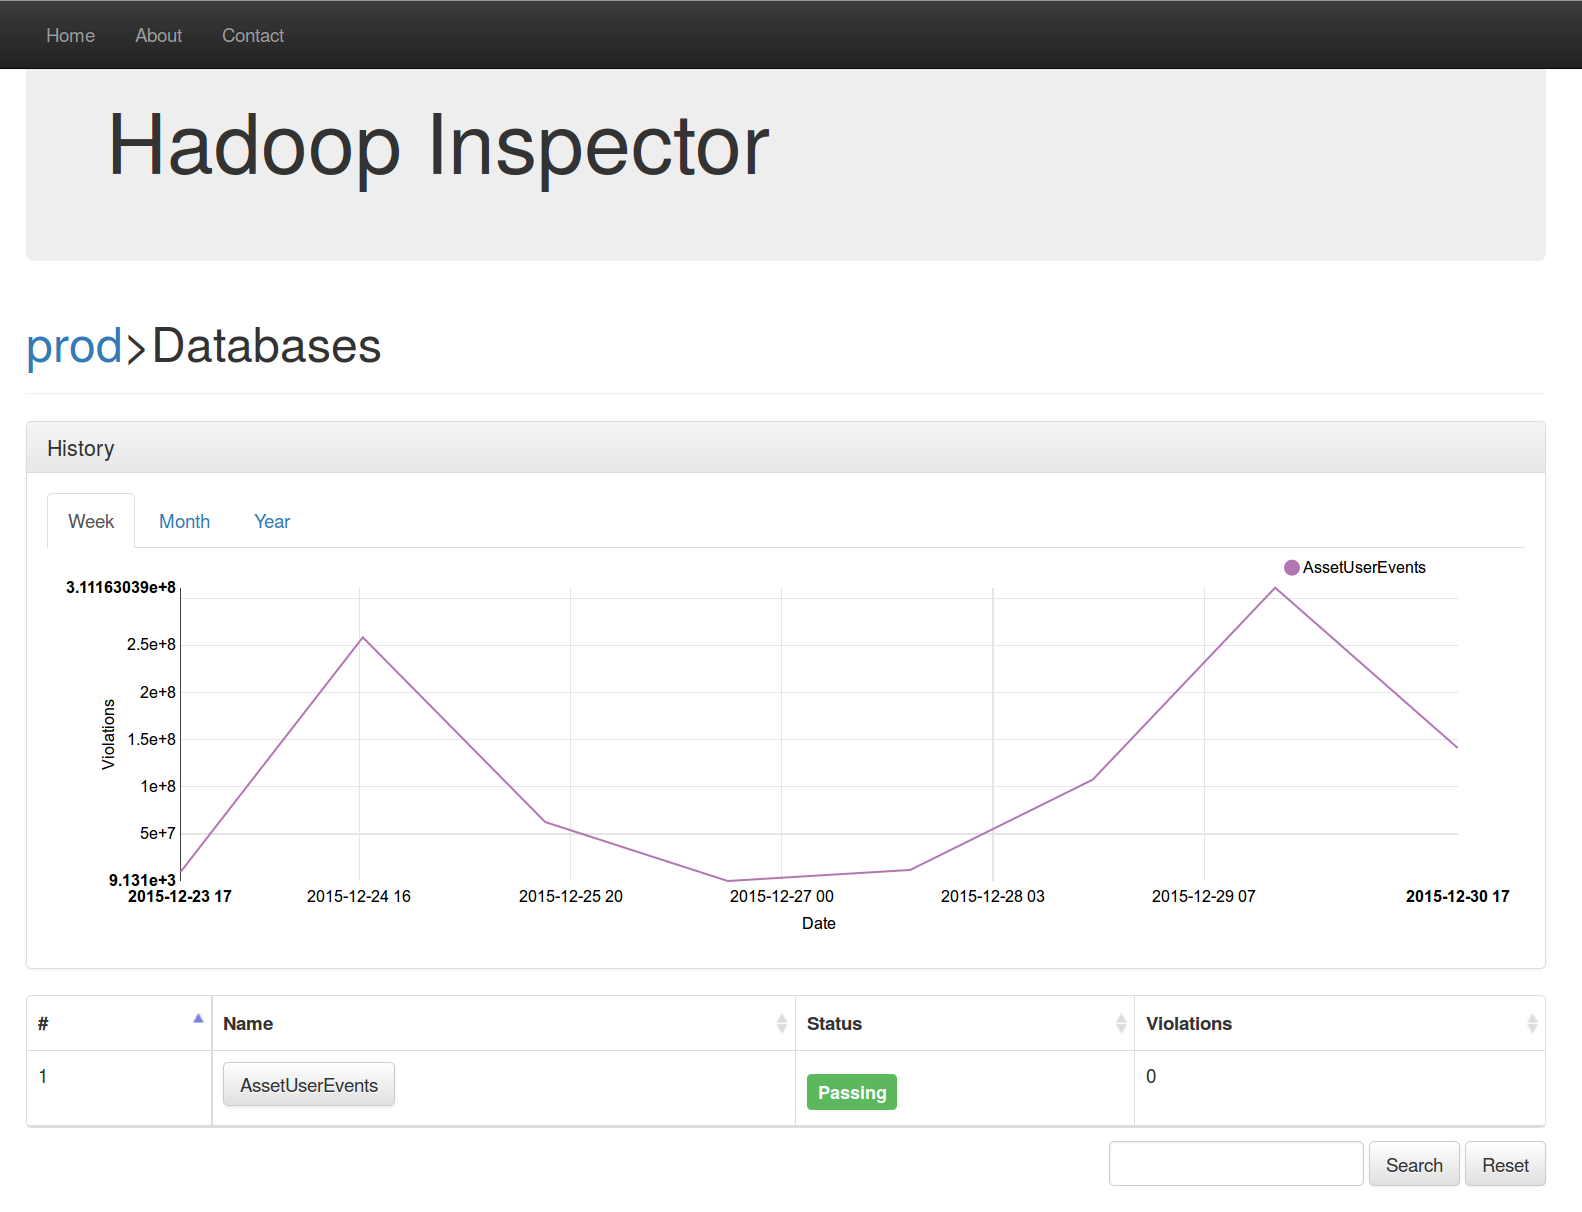
\includegraphics[width=\textwidth]{screen1.png}
\end{figure}
\end{minipage}\hfill % End the sidebar mini page 
%
%----------------------------------------------------------------------------------------
%	MAIN BODY - FIRST PAGE
%----------------------------------------------------------------------------------------
%
\begin{minipage}[c]{.32\linewidth}
\begin{mdframed}[style=sidebar,frametitle={}] % Sidebar box

{\large
\begin{centering}
    \textbf{Sample Check Types}
\end{centering}
}

\centerline {\rule{.75\linewidth}{.25pt}} % Horizontal line

\NewList
\ListProperties(Style1=\bfseries,Style1*=$\bullet$ ,Hide1=1)
\ListProperties(Style2*=-- ,Hide2=2)
\ListProperties(Margin1=0cm,Margin2=0.1cm)
\ListProperties(Space=-0.1cm,Space*=-0.1cm)
\begin{easylist}
    @ Data Quality Checks:
    @@ check uniqueness
    @@ check foreign key reference
    @@ check case
    @@ check min and max value
    @@ check min and max length
    @@ check accessibility
    @@ check type
    @@ check required fields
    @@ check unknown value
    @@ check enumerated value
    @@ check {\ttfamily start\_timestamp} < {\ttfamily stop\_timestamp}
    @ Data Consistency Checks
    @@ check base vs summary table
    @@ check peer tables
    @@ check target vs source
    @ Data Management Checks:
    @@ check statistics age
    @@ check retention age
    @@ check access
    @@ check blocksize
    @@ check file formats
\end{easylist}

\end{mdframed}
\end{minipage} % End the main body - first page mini page

%----------------------------------------------------------------------------------------
%	MAIN BODY - SECOND PAGE
%----------------------------------------------------------------------------------------

\begin{minipage}[t]{.66\linewidth} % Mini page taking up 66% of the actual page

\heading{Architecture}{0pt}

\NewList
\ListProperties(Style1=\bfseries,Style1*=$\bullet$ ,Hide1=1)
\ListProperties(Style2*=-- ,Hide2=2)
\ListProperties(Style3*=$\bullet$ ,Hide3=3)
\ListProperties(Margin1=0cm,Margin2=0.4cm,Margin3=1cm)
\ListProperties(Space=0cm,Space*=0cm)
\begin{easylist}
    @ Reusable and Flexible Plug-in Architecture
    @@ Phase One: Universal Plug-ins
    @@@ checks are written in any language
    @@@ runner passes run-time info to checks via env vars
    @@@ checks pass results back to runner via stdout
    @@ Phase Two: SQL Plug-ins
    @@@ checks are written as SQL
    @@@ checks are a template that is filled-in by runner
    @@ Phase Three: Native Plug-ins
    @@@ checks are written as Python modules
    @@@ checks inherit from one another
    @@@ runner imports plug-ins, has tight exception handling, logging, etc
    @ Check Results Database to support historical forensics and data annotation.
    @ Both rule and profiling checks
    @ Version-control-compatible checks and registry - allowing test code to be managed with DDL.
\end{easylist}

%\heading{Frequently Asked Questions}{0pt}

%\centerline {\rule{.75\linewidth}{.25pt}} % Horizontal line
%
%\textbf{Q1: Why test data at rest rather than before it gets to Hadoop?}
%
%Answer: data should be tested in both places, but it can be most reliably and
%effectively tested within its target location since Hadoop has more ways of
%expressing a test against data at rest than ETL processes have, and have access
%to all data that's been loaded, not just a single batch. Specifically:
%
%\begin{itemize}
%    \item Testing of uniqueness and completeness doesn't work as well in the
%ETL process since a tested-file may get loaded twice, dropped before load, or
%in the case of uniqueness may require analysis of multiple batches.
%    \item Testing of data distributions can be problematic within ETL since the
%distribution problem may not be revealed until enough data has been processed
%that some has already been loaded.
%    \item Policy testing doesn't even apply to ETL at all. This includes
%directory, file and table naming conventions, ownership, file types,
%compression, security, completeness and freshness of stats, etc.
%    \item Certain types of tests are difficult to write and get good
%performance for within ETL - like foreign key constraints across two tables.
%    \item Consistency testing between two peer tables (ex: for failover in two
%separate clusters) with a single ETL process loaded data into one - isn't even
%possible.
%\end{itemize}
%
%\textbf{Q2: What types of tests should still be performed within the ETL process?}
%
%Answer: since the cost of repair is generally lower when invalid data is caught
%by the ETL, whatever can be effectively tested at that stage should be. This
%includes, for example:
%
%\begin{itemize}
%    \item Testing of logic conditions completely contained within a single batch of data
%    \item Testing of field formats, lengths, valid values, unknown values, min and max values, etc
%    \item Testing of foreign key relationships when practical
%\end{itemize}
%
%\textbf{Q3: Why not write all test results directly into Hadoop rather than SQLite?}
%
%Answer: it will eventually, for now, for the sake of development speed, we're writing to SQLite

\vspace{0.5cm}

\heading{Licensing}{0pt}

\centerline {\rule{.75\linewidth}{.25pt}} % Horizontal line

Hadoop Inspector is protected by the BSD license.  See the file "LICENSE" in
the source code root directory for the full language or refer to it here:
\href{http://opensource.org/licenses/BSD-3-Clause}{http://opensource.org/licenses/BSD-3-Clause}\\
Copyright 2015 Will Farmer and Ken Farmer

\end{minipage}\hfill % End of the main body - second page mini page
\begin{minipage}[t]{.30\linewidth} % Mini page taking up 30% of the actual page

%----------------------------------------------------------------------------------------
%	SIDEBAR - SECOND PAGE
%----------------------------------------------------------------------------------------

\begin{mdframed}[style=sidebar,frametitle={}] % Sidebar box

\heading{Roadmap}{0pt}

\centerline {\rule{.75\linewidth}{.25pt}} % Horizontal line

\NewList
\ListProperties(Style1=\bfseries,Style1*=$\bullet$ ,Hide1=1)
\ListProperties(Style2*=-- ,Hide2=2)
\ListProperties(Margin1=0cm,Margin2=0.1cm)
\ListProperties(Space=-0.1cm,Space*=-0.1cm)
\begin{easylist}
    @ 2015-10-01:\\Initial Release
    @@ Runner: initial release
    @@ Web Server: initial release
    @ 2015-11-01:\\Solidification
    @ 2015-12-01:\\Functionality
    @@ Support for native-SQL checks
    @ Future
\end{easylist}

\end{mdframed}\hfill

\centering
\begin{minipage}[t]{.95\linewidth}
\textbf{Contact Information:}\\
Will Farmer, Ken Farmer\\
\href{mailto:willzfarmer@gmail.com}{willzfarmer@gmail.com}\\
\href{www.will-farmer.com}{www.will-farmer.com}\\
\href{mailto:kenfar@gmail.com}{kenfar@gmail.com}\\
\href{www.linkedin.com/in/kenfar}{www.linkedin.com/in/kenfar}
\end{minipage}

\end{minipage} % End of the sidebar mini page

%----------------------------------------------------------------------------------------

\end{document} 
